\section*{Assignment 09: Scaling Strategy}
\addcontentsline{toc}{section}{Assignment 09: Scaling Strategy}

For SkillSync we face three scaling stages. Phase one is product-market fit: fortify the core, test network effects within a single geographic cluster, and land two local anchor partners (trade association plus municipal innovation unit) because their signalling power lifts both sides simultaneously \citep{Choudary2016,Reillier2017}. During this phase we need a focused growth pod, two developers dedicated to stable operations, and a community manager who moderates feedback loops inside our pilot Slack.

Phase two tackles regional scaling. We standardise onboarding flows and API contracts so new partners can plug in without constant hand-holding. A three-tier partner programme (community, certified, strategic) gives us a lever to manage quality while offering incentives to invest in integrations \citep{HagiuWright2013}. We staff a lean partner-success team, ship shared dashboards, and track cross-side conversion plus time-to-value per partner to monitor whether network effects accelerate \citep{ShapiroVarian1999}.

\begin{figure}[h]
  \centering
  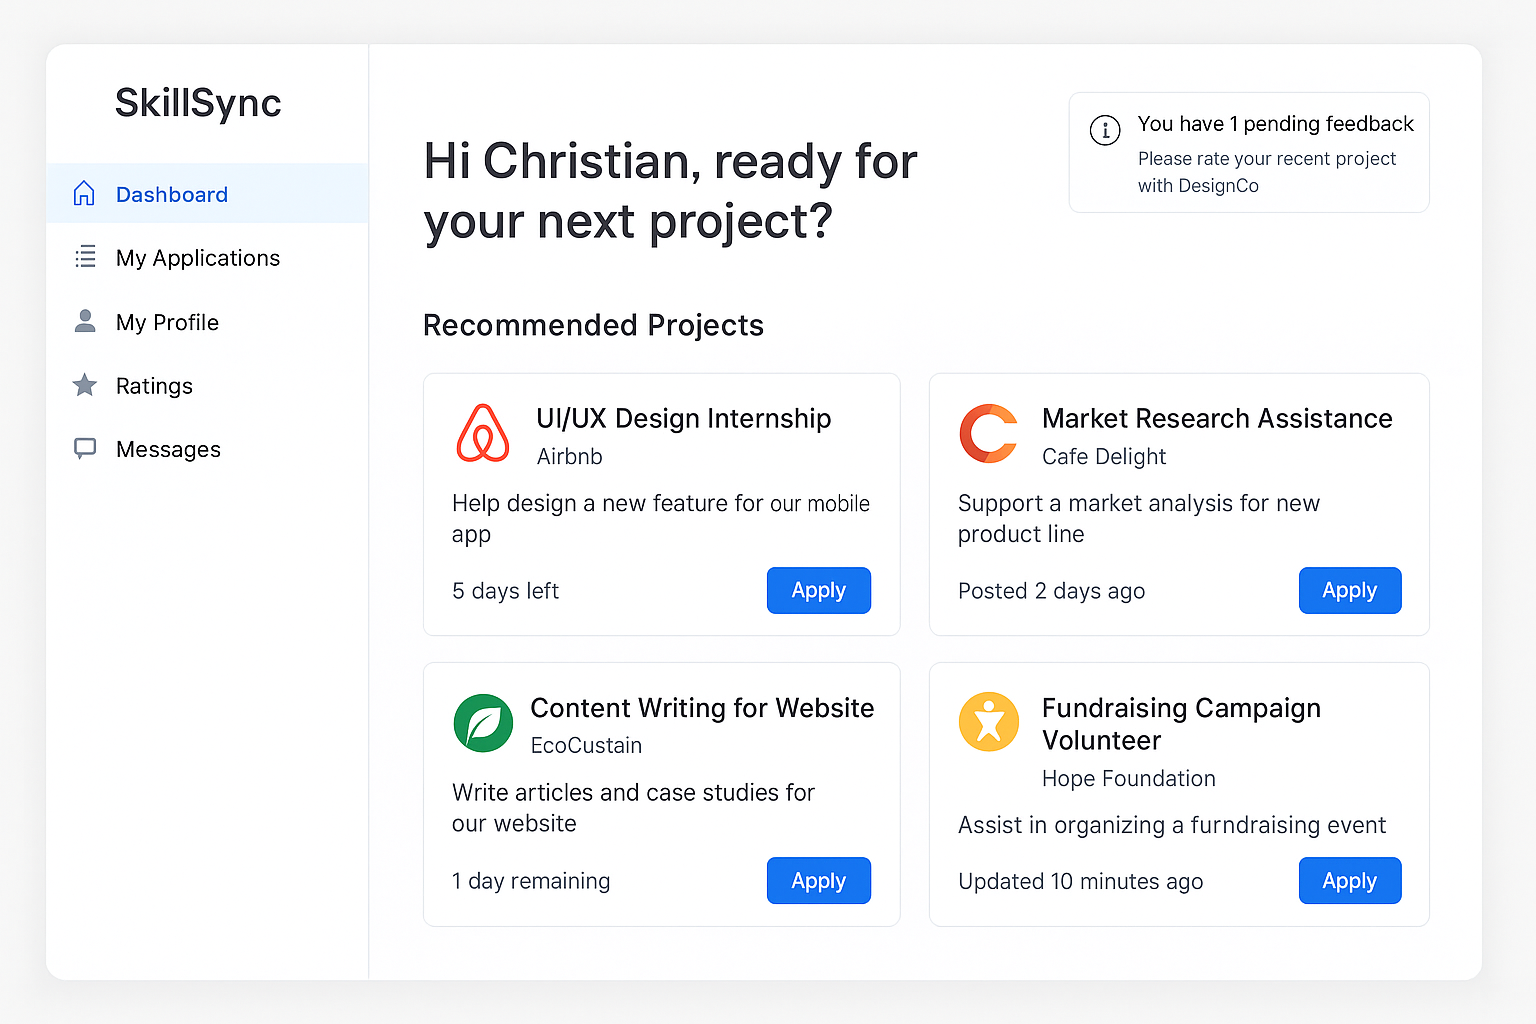
\includegraphics[width=0.75\linewidth]{figures/opgave09/Dashboard.png}
  \caption{Adoption dashboard mock-up from `Dashboard.png` tracking activation once partner enablement becomes self-serve.}
  \label{fig:scaling-dashboard}
\end{figure}

Figure~\ref{fig:scaling-dashboard} (based on `Dashboard.png`) keeps the SkillSync crew honest by showing how activation rates inflect only after partner enablement becomes self-serve, so we resist the temptation to sprint ahead until the curve bends.

Phase three moves national (maybe Nordic) but only if the first two phases prove positive unit economics. We court alliances with larger institutional players and negotiate white-label deals with select enterprise clients. Governance must expand with clear data-sharing principles, algorithm audits, and an advisory board so legitimacy scales \citep{Srnicek2017,Zuboff2019}. We also budget for compliance expertise, localisation, and a small deal desk that can tailor partnerships without wrecking the standard product.

Rolling out the plan exposes two main risks: churn and quality decay. Churn can hit both users and partners, especially if competitors tempt them with exclusive features or lower fees. To counteract that we build switching costs through data portability (export and import of history), loyalty loops, and analytics that lose value if someone leaves \citep{FarrellSaloner1986,ShapiroVarian1999}. Quality decay typically shows up when rapid growth dilutes standards. The antidote is a clear set of service-level agreements, automated monitoring of match quality, and quarterly partner reviews where we can suspend actors who under-deliver \citep{Reillier2017}. I also loop in a community review board to catch soft signals before the dashboards scream.

The theory lines up with classic platform literature: network effects demand critical mass, but pushing too fast can erode match quality, which Porter would note reduces differentiation \citep{Porter2008}. \citet{Choudary2016} remind us that governance and producer-enablement tools must evolve alongside scaling phases or we run out of trust. \citet{Srnicek2017} adds that data-driven platforms only stay powerful when they pair aggressive growth with legitimacy and transparency, which is why I invest so much energy in the partnership programme and organisational scaffolding.

To stress-test the roadmap we built a simple simulation model in Google Sheets. Inputs include activation rate, partner acquisition velocity, moderation load, and average project value. We used it to sanity-check how many moderators and partner managers we need per 1,000 active users and to plan the budget buffer for unexpected churn. The model also highlighted when to pause expansion: if quality scores drop below 4.4/5 for two consecutive months, we freeze new partner intake until the governance board signs off on remediation. Those thresholds feed into the admin panel described in Assignment~05.

To keep the scaling journey humane, every phase ends with a ``story harvest'' where students, NGOs, and team members share what surprised them. Those stories feed marketing assets and internal training so the team stays grounded in impact. Quarterly retros using \citet{Choudary2016}'s interaction-model canvas remind us the platform is a living system.
